\documentclass{article}

\usepackage[T1]{fontenc}
\usepackage{amsmath, amsthm}
\usepackage{amssymb}
\usepackage{listings}
\usepackage[svgnames]{xcolor}
\usepackage{tikz}
\usepackage{array}
\usepackage{graphicx}
\usepackage[backend=biber, maxbibnames=9]{biblatex}
\usepackage{algpseudocode}
\usepackage{algorithm}
\usepackage{mathtools}
\usepackage{xcolor}
\usepackage{subcaption}
\usepackage{wrapfig}
\usepackage{hyperref}

\newcommand{\Set}[2]{%
  \{\, #1 \mid #2 \, \}%
}

\makeatletter
\newcommand{\superimpose}[2]{{%
  \ooalign{%
    \hfil$\m@th#1\@firstoftwo#2$\hfil\cr
    \hfil$\m@th#1\@secondoftwo#2$\hfil\cr
  }%
}}
\makeatother

\newcommand{\leftplus}{\mathbin{\mathpalette\superimpose{{\leftarrow}{+}}}}
\newcommand{\disquare}{\mathbin{\text{\tikz [x=1ex,y=1ex,line width=.1ex,line join=round] \draw (0,0) rectangle (1,1) (.5\pgflinewidth,.5) -- (.5,1ex-.5\pgflinewidth) -- (1ex-.5\pgflinewidth,.5) -- (.5,.5\pgflinewidth) -- (.5\pgflinewidth,.5) -- cycle;}}}

\graphicspath{{./images/}}

% NOTE: need to run `biber report` to ensure up-to-date references
\addbibresource{report.bib}

\title{The Beginnings of an Optimizing Compiler for a Very High Level Language}
\author{Anthony Hunt}

\begin{document}
\maketitle
\tableofcontents
\newpage

\section{Introduction}

In the modern era of programming, optimizing compilers must make aggressive choices in pursuit of the most efficient, yet correct, representation of source code. For low level languages like C and Rust, automatic optimizations on-par with human abilities are a mature part of the software ecosystem and a reasonable expectation for performance-oriented programmers. The effectiveness of a compiler directly influences the contributors and community of its source language, providing sweeping benefits across entire codebases at minimal cost.

However, in domains that do not require peak efficiency, high level languages focused on readability and ease-of-use have become foundational. As software development continues to grow more accessible to the general public, the responsibilities of compilers to shoulder the burden of optimization are even more pronounced. Languages like Python and JavaScript have numerous libraries and runtimes that are built on efficient languages but expose only easy-to-use, native APIs.

In the last two papers of this series, we explored a collection of abstract data types in practice and recent research into term rewriting systems for optimizing compilers. Now, we turn our attention to a prototypical implementation of a very high level language, usable by expressive discrete math notation and built with the efficiency of a low-level language. Although we do not present a full compiler as of yet, we discuss a few critical findings that will serve well in a long-term implementation.

The rest of this paper explores theoretical optimizations on select examples, a few implementation tests, then outlines a roadmap for a full compiler implementation.

\section{Exploring Examples}

Optimizations-by-example are effective in probing a domain for natural language designs, common expressions, and current pain points. As the novelty of our language stems from its emphasis of abstract data types for modelling using sets, sequences, and relations, the following examples aim to cover a sufficient amount of real-world usage for which we focus our design and optimization efforts.

\subsection{The Birthday Book Problem}

An older paper by Spivey \cite{spivey1989birthday} outlines a simple but fitting modelling problem we now explore at length: A birthday book tracks the relationship between the names of people and their birthdays. All names are assumed to be unique, yet two or more people may share the same birthday. Using this book, we attempt to answer two main questions:
\begin{itemize}
  \item When is the birthday of a particular person?
  \item Who has a birthday on a given date?
\end{itemize}
These questions correspond to the lookup and reverse lookup tasks on a set of relations. In other words, to find the birthday of a person, we require a function $lookup: Name \rightarrow Date$. Likewise, we denote $lookup^{-1}: Date \rightarrow \{Name\}$, which returns a set of names that are born on a specific date. Then, our high level language should provide an optimized version of these functions that returns from $lookup$ or $lookup^{-1}$ as fast as possible.

\subsubsection{Handling Relations: Many-to-One and Many-to-Many}

The relational data structure of this question involves a many-to-one correspondence, where many names can map to the same date. In many programming languages, a straightforward method of modelling the data is to maintain two dictionaries, one for regular lookups and another for reverse lookups. As a more concrete example, let $birthday\_book$ denote an example relation of birthday book items, where keys are names and dates are represented by integers. A mapping of this book would be stored as:
\[birthday\_book = \{\text{Alice} \mapsto 25, \text{Bob} \mapsto 30, \text{Charlie} \mapsto 35, \text{Kevin} \mapsto 35 \}\]
Then, the reverse mapping could be stored like so:
\[birthday\_book^{-1} = \{25 \mapsto \text{Alice}, 30 \mapsto \text{Bob}, 35 \mapsto [\text{Charlie, Kevin}] \}\]
Lookups and inverse lookups would search through these dictionaries as a hashmap accordingly.

When implemented in Python, this method performs well on small data types, but has the undesirable consequence of maintaining two sets of duplicated data for all operations. This duplication is especially inefficient for entries that contain large quantities of data, like nested records or tuples. For example, if Kevin were to be removed from the birthday book, both the regular birthday book dictionary and the list of names in the inverse dictionary would need to be modified.

To eliminate some of the duplicated data, we could instead transform the keys of one of the dictionaries to use pre-hashed values directly. For example, consider a hash function $h(x)$ that happens to return the following, provided our input of names:
\begin{align*}
h(\text{Alice}) &= 0\\
h(\text{Bob}) &= 1\\
h(\text{Charlie}) &= 2\\
h(\text{Kevin}) &= 3\\
\end{align*}
Further, let $collision\_resolver$ be some reasonable but deterministic hash collision resolution function. Then, the birthday book dictionary can contain the following entries, with hashes in place of names:
\[birthday\_book = \{0 \mapsto 25, 1 \mapsto 30, 2 \mapsto 35, 3 \mapsto 35 \}\]
To resolve any collisions from our pre-hash function $h$, we can define a modified lookup function as in Algorithm~\ref{fig:birthdayLookup}.

\begin{algorithm}
  \caption{$lookup$ using a pre-hashed dictionary}
  \begin{algorithmic}
    \Require $n: \text{Name}$
    \State $hash\_name \gets h(n)$
    \While{True}
      \State $possible\_date \gets birthday\_book[hash\_name]$
      \If{$possible\_date = None$}
        \Return $None$
      \EndIf
      \State $names\_for\_date \gets lookup^{-1}(possible\_date)$
      \If{$n \in names\_for\_date$}
        \Return $possible\_date$
      \EndIf
      \State $hash\_name \gets collision\_resolver(hash\_name)$
    \EndWhile
  \end{algorithmic}
  \label{fig:birthdayLookup}
\end{algorithm}

By keeping one complete dictionary, the other can rely on cross-dictionary lookups to resolve hashing collisions. Unfortunately, we still need to duplicate at least one set of either names or dates to resolve hashing collisions, but for larger data types, this method could use 25\% less space with a little runtime cost.

Similar data structures with less overhead and clever elimination of duplicated data via pointers could prove useful in providing O(1) reverse lookups. For example, C++'s Boost.Bimap library \cite{boostBimap1, boostBimap2} stores pairs of values and provides efficient views for both forward and reverse lookups, with the caveat that the relation must be one-to-one. Alternatively, a post on StackOverflow \cite{bimapStackOverflow} describes a solution with two maps of values to pointers (with types $A \rightarrow B*$ and $B \rightarrow A*$). In this case, data is stored in two sets of pairs that couple a concrete value with its opposing pointer. Then, the $lookup$ function can dereference the pointer received from the $A \rightarrow B*$ to find the concrete value of $B$ stored in the second set.

\subsubsection{Extending the Problem with Two Birthday Books}
Extending the problem, we demonstrate the ergonomics of set operators over real world models. With consideration for the bidirectional mapping setup from the previous questions, we seek to efficiently implement the following scenarios:
\begin{enumerate}
  \item Two groups of friends become acquainted, each with an originally independent birthday book. Eventually, they wish to merge their records together, removing duplicate entries for mutual friends.
  \item A subset of the original friend group eventually have a falling out and wish to separate from the main group. This problem then requires one birthday book to be separated into two.
  \item When planning for a birthday party, the group wants to acknowledge not only the person's birthday, but any and all national holidays associated with that day.
\end{enumerate}

A straightforward model for the first scene would assume that two groups $A$ and $B$ have an existing birthday book. Then the new birthday book will consist of the union of these two relations. Keeping in mind the invariant that names within friend groups must remain unique, the new set $C$ can be constructed as in Algorithm~\ref{fig:birthdayUnion}.
\begin{algorithm}
  \caption{Birthday Book Union}
  \begin{algorithmic}
    \Require $A, B: \text{Name} \times \text{Date}$
    \State $C \gets A$
    \For{$b \in B$}
      \If{$b.name \notin A$}
        \State $C.add(b)$
      \EndIf
    \EndFor\\
    \Return $C$
  \end{algorithmic}
  \label{fig:birthdayUnion}
\end{algorithm}

The second setting could be resolved through a set difference of the small friend group from the large friend group. Let $L$ be the remaining friends from the group separation. Then, Algorithm~\ref{fig:birthdaySep} contains the corresponding programmatic model.
\begin{algorithm}
  \caption{Birthday Book Separation}
  \begin{algorithmic}
    \Require $A, B: \text{Name} \times \text{Date}$
    \State $L \gets \{\}$
    \For{$a \in A$}
      \If{$a.name \notin B$}
        \State $L.add(a)$
      \EndIf
    \EndFor\\
    \Return $L$
  \end{algorithmic}
  \label{fig:birthdaySep}
\end{algorithm}

Finally, the third situation could be expressed through the composition of two relations. Let $H: Holiday \times Date$ be a relation of holidays to their respective dates. Then, those people who have a birthday from set $A$ coinciding with a holiday may be found by $C = A\mathbin{;}H^{-1}$. Corresponding code is shown in Algorithm~\ref{fig:birthdayComp}.

\begin{algorithm}
  \caption{Birthday Book Composition}
  \begin{algorithmic}
    \Require $A: \text{Name} \times \text{Date}, H: \text{Holiday} \times \text{Date}$
    \State $C \gets \{\}$
    \For{$a \in A$}
      \State $h \gets H.lookup^{-1}(a.date)$
      \If{$h \neq None$}
        \State $C.add(\langle a.name, h.holiday \rangle)$
      \EndIf
    \EndFor\\
    \Return $C$
  \end{algorithmic}
  \label{fig:birthdayComp}
\end{algorithm}

\subsection{Other Combinations of Sets, Sequences, and Relations}

In general, the feasibility of an efficient compiler for a very high level language relies on the idea that rewrite rules combined with efficient implementations of data types will reduce the runtime of complex set manipulation expressions. Dissecting several examples from a catalogue of Event B models revealed that the most common modelling expressions make use of conditions on sets, unions, intersections, and differences. Because the implementation of sets is the least constrained out of the ``collection'' types, we focus optimization efforts on manipulating those implementations for more efficient results.

Set construction notation of the form $\Set{elem}{generators: conditions}$ (eg. $\Set{x}{x \in S : x > 0}$) appears often when dealing with models founded on discrete math. Further, operations on sets, like union, intersection, and difference, can be rewritten in set construction form:
\begin{align*}
  S \cup T &= \Set{x}{x \in S \lor x \in T}\\
  S \cap T &= \Set{x}{x \in S \land x \in T}\\
  S \setminus T &= \Set{x}{x \in S \land \lnot x \in T}
\end{align*}
Theoretically, using the lower-level boolean forms of these expressions should enable cleverer forms of execution that prevent unnecessary set constructions, either by way of lazy evaluation or condition manipulation.

In Python, set construction for the most part translates to a set comprehension of the form \texttt{\{elem for elem in iterable if <condition>\}} (eg. \texttt{\{x for x in S if x > 0\}}). Additionally, operators for union, intersection, and difference are \texttt{|}, \texttt{\&}, and \texttt{-}.

We now list a few simple but common examples of set-based expression optimizations:
\begin{itemize}
  \item A function $f$ applied over the difference of two sets may be written in a modelling language as $\Set{f(x)}{x \in S \setminus T}$. Translated to more Python-like syntax, this becomes \texttt{\{f(x) for x in S - T\}}. The default implementation of such an expression, with no knowledge over the side effects of $S$, $T$, and $f$, would first construct a temporary set \texttt{text = S - T}, then perform \texttt{\{f(x) for x in temp\}}. However, a more efficient implementation would rewrite the initial expression to \texttt{\{f(x) for x in S if x not in T\}}, effectively trading the overhead of temporary set construction for $|S|$ $O(1)$ lookup operations.
  \item Mapping over a difference of sets $S \setminus T$ where $|T| << |S|$ could also be performed by successive \texttt{[S.pop(x) for x in T]} operations, mutating $S$ directly and avoiding another set construction. An implementation of \texttt{pop} could also move selected elements to one end of the list and keep track of an index of ``deleted'' elements for future operations. Likewise, $S \cup T$ with $|T| << |S|$ may be serviced with sequential \texttt{add} operations
  \item A similar index tracking idea could be used for sets that ``consume'' another set. For example, consider Algorithm~\ref{fig:prodcons}, where $P$ and $C$ represent a producer and consumer set respectively. The $P$ set may be needed elsewhere in the code, so we cannot destroy its contents to build $C$. In this case, internally representing $P$ as an array of ordered elements and $C$ as an index into the first $n$ elements of $P$ will be suitable. New elements are appended to the list representation of $P$ (assuming no duplicates), so the addition and consumption of elements remain completely isolated while reducing duplicate data and repeated set constructions.
  \item Early stopping in quantification based expressions. For example, the statement $\forall x \mid x \in S \cap T \land p(x)$ would normally require construction of an intermediate set for $S \cap T$ and then a loop to check the property of all resulting elements. However, we do not necessarily need to construct any sets in this question. Instead, we can combine all terms into a single for-loop over only one of the sets, as seen in Algorithm~\ref{fig:earlyStoppingQuant}. Similar set manipulations can be used for existential quantification.
\end{itemize}

\begin{algorithm}[h]
  \caption{Set Producer-Consumer}
  \begin{algorithmic}
    \Require $P: Set, C: Set, C = \emptyset$
    \While{$|P| \neq |C|$}
      \State $e \gets (P - C).pop()$
      ... \Comment{Function body, $P, C$ read but not modified}
      \State $C \gets C \cup {e}$
      \State $P \gets P \cup {n}$ ... \Comment{$P$ may produce new elements}
    \EndWhile
  \end{algorithmic}
  \label{fig:prodcons}
\end{algorithm}

\begin{algorithm}[h]
  \caption{Early Stopping for Universal Quantification over Intersection}
  \begin{algorithmic}
    \Require $S, T, p$
    \State $M \gets min(S,T)$ \Comment{$min$ compares the number of elements in a set}
    \For{$x \in M$}
      \If $\lnot(x \in T \land p(x))$
        \Return $false$
      \EndIf
    \EndFor\\
    \Return $true$
  \end{algorithmic}
  \label{fig:earlyStoppingQuant}
\end{algorithm}

Different flavours of optimizations for complex expressions and other ``collection'' data types will be added as needed, but the deep static analysis and code awareness is evidently integral to the optimization process. In the next section, we discuss a rewrite system to facilitate the optimization process.

% the concepts of such a language, an optimization process, and an interface for continuous, extendable optimizations.

\section{A TRS for a Very High Level Language}
\subsection{Rewriting Rules for Set Notation}

In Section 2, we presented a selection of examples wherein expressive set notation for modelling could be rewritten for efficient code generation. Now, we extend this collection to optimize generic combinations of set operators as a complete collection of set-oriented rewrite rules. As we derive this system, assume each iterable data type holds efficient representations of size calculation and set membership.

To simplify all terms in the rewrite system, we introduce a rule to exhaustively reduce sets into set construction notation. Note that for all rules, capital letters represent sets and lowercase for elements and functions:
\begin{equation}
S \rightarrow \Set{x}{x \in S}
\end{equation}
Then, our basic operators $\cup, \cap, \setminus$ can be reduced to combined construction notation with boolean conditions:
\begin{align}
  \Set{x}{x \in S} \cup \Set{y}{y \in T} &\rightarrow \Set{x}{x \in S \lor x \in T}\\
  \Set{x}{x \in S} \cap \Set{y}{y \in T} &\rightarrow \Set{x}{x \in S \land x \in T}\\
  \Set{x}{x \in S} \setminus \Set{y}{y \in T} &\rightarrow \Set{x}{x \in S \land x \notin T}
\end{align}
A proof of correctness for these types of rules is directly given by the definition of each operator and variable substitution. We present the proof of union below, recognizing similar forms for intersection and set difference:
\begin{proof}
  \begin{align*}
    &S \cup T\\
    =&\Set{x}{x \in S} \cup \Set{y}{y \in T}\\
    =&\Set{z}{(x \in S \land x = z) \lor (y \in T \land y = z)}\\
    =&\Set{z}{z \in S \lor (y \in T \land y = z)}\\
    =&\Set{z}{z \in S \lor z \in T}\\
    =&\Set{x}{x \in S \lor x \in T}\\
  \end{align*}
\end{proof}
Although the proof is relatively simple, such proofs are of particular importance to ensuring correctness of variables used within one another. A generalized form of these rules, involving additional predicates $p,q: Any \rightarrow Boolean$, may be required. We observe that predicates joined to a generator $x\in S$ with $\lor$ are malformed, since any $x$ satisfying the predicate may be valid.
\begin{align}
  \Set{x}{x \in S \land p(x)} \cup \Set{y}{y \in T \land q(y)} &\rightarrow \Set{x}{(x \in S \land p(x)) \lor (x \in T  \land q(x))}\\
  \Set{x}{x \in S \land p(x)} \cap \Set{y}{y \in T \land q(y)} &\rightarrow \Set{x}{x \in S \land x \in T \land p(x) \land q(x)}\\
  \Set{x}{x \in S \land p(x)} \setminus \Set{y}{y \in T \land q(y)} &\rightarrow \Set{x}{x \in S \land x \notin T \land p(x) \land q(x)}
\end{align}

Often times, we find that functions are applied to the generated elements, similar to $\Set{f(x)}{x \in S}$. The above operator-based rules can therefore be expressed as:
\begin{align}
  \Set{f(x)}{x \in S} \cup \Set{y}{y \in T} &\rightarrow \Set{f(x)}{x \in S \lor f(x) \in T}\\
  \Set{f(x)}{x \in S} \cap \Set{y}{y \in T} &\rightarrow \Set{f(x)}{x \in S \land f(x) \in T}\\
  \Set{f(x)}{x \in S} \setminus \Set{y}{y \in T} &\rightarrow \Set{f(x)}{x \in S \land f(x) \notin T}
\end{align}

A further generic form might be considered for sets built from mapped-over operands. However, the lack of relationship between a function mapped over the first set versus a different function mapped over the second set restricts the amount of feasible algebraic manipulation. In this case, we first evaluate one operation fully to then apply one of the rules in the previous paragraph. Note that unions of this form gain no tangible benefit from an extra set construction, so we opt to join entries together as seen in the partial derivation of rewrite rule 11. An optional predicate within each set construction may be carried through the rewrite rule as seen in equations 5-7, but for conciseness, we omit these rules for now.
\begin{align}
  \Set{f(x)}{x \in S} \cup \Set{g(y)}{y \in T} &\rightarrow
    \begin{split}
      \Set{z}{&(x \in S \land f(x) = z) \\\lor &(y \in T \land g(y) = z)}
    \end{split}\\
  \Set{f(x)}{x \in S} \cap \Set{g(y)}{y \in T} &\rightarrow
    \begin{split}
      &T_2 := \Set{g(y)}{y \in T};\\
      &\Set{f(x)}{x \in S} \cap \Set{y}{y \in T_2}
    \end{split}\\
  \Set{f(x)}{x \in S} \setminus \Set{g(y)}{y \in T} &\rightarrow
    \begin{split}
      &T_2 := \Set{g(y)}{y \in T};\\
      &\Set{f(x)}{x \in S} \setminus \Set{y}{y \in T_2}
    \end{split}
\end{align}

Additionally, a few specialized cases arise when the function $f$ is injective and identical between set constructions. Further predicate clauses (as seen in equations 5-7) may be brought over as above and renamed as functions of $x$.
\begin{align}
  \Set{f(x)}{x \in S} \cup \Set{f(y)}{y \in T} &\rightarrow \Set{f(x)}{x \in S \lor x \in T}\\
  \Set{f(x)}{x \in S} \cap \Set{f(y)}{y \in T} &\rightarrow \Set{f(x)}{x \in S \land x \in T}\\
  \Set{f(x)}{x \in S} \setminus \Set{f(y)}{y \in T} &\rightarrow \Set{f(x)}{x \in S \land x \notin T}
\end{align}

In targeting expressions that make use of set operators nested within set constructors, like $\Set{x}{x \in f(S, T)}$, we create the following rules:
\begin{align}
  \Set{x}{x \in \Set{y}{y \in S}} &\rightarrow \Set{x}{x \in S}\\
  \Set{x}{x \in \Set{y}{y \in S \land p(x)} \land q(x)} &\rightarrow \Set{x}{x \in S \land p(x) \land q(x)}\\
  \Set{x}{x \in \Set{y}{y \in S \land p(x)}} &\rightarrow \Set{x}{x \in S \land p(x)}\\
  \Set{x}{x \in \Set{y}{y \in S} \land q(x)} &\rightarrow \Set{x}{x \in S \land q(x)}
\end{align}

Finally, we can now target the boolean statements within set constructions. However, we first give some intuition towards the overarching principles behind non-trivial terms. Generally, breaking down each operation into set builder notation enables us to perform the following actions:
\begin{itemize}
  \item One membership operator within each set of ``and''-clauses will act as an element generator. Then, other clauses will act as conditions for an internal if-statement. For example, if the rewrite system observes an intersection of the form $\Set{x}{x \in S \land x \in T}$, the set construction operation must iterate over at least one of $S$ and $T$. Then, the other will act as a condition to check every iteration.
  \item A collection of ``or''-clauses will generally be split into multiple sequential loops. Therefore, each clause must contain at least one element generator. Any ``and''-clauses nested within a single top-level ``or''-clause group will then act as a condition as specified above.
  \item Generators must be statements of the form $x \in S$, where $x$ is used in the ``element'' portion of the set construction. Statements like $x \notin T$ or checking a property $p(x)$ must act like conditions since they do not produce any iterable elements.
  \item Any boolean expression for conditions may be rewritten as a combination of $\lnot, \lor$, and $\land$ expressions. Therefore, by converting all set notation down into boolean notation and then generating code based on set constructor booleans, we can accommodate any form of predicate function.
\end{itemize}

The following rules formalize this intuition, where generators $S$ (and $T$ when needed) are the smallest sets within a local ``and''-clause:
\begin{align}
  % Should these first two break down into pieces that can be handled by the third rule here? The TRS may not terminate though...
  \Set{f(x)}{(x \in S \land p(x)) \lor (x \in T \land q(x))} &\rightarrow \text{Algorithm~\ref{fig:eq15alg}}\\
  \Set{z}{(x \in S \land f(x) = z \land p(x)) \lor (y \in T \land g(y) = z \land q(y))} &\rightarrow \text{Algorithm~\ref{fig:eq16alg}}\\
  \Set{f(x)}{x \in S \land p(x)} &\rightarrow \text{Algorithm~\ref{fig:eq17alg}}
\end{align}
And a specialized version of equation 21, preferring the use of intersections to reduce duplicate ``or''-clause loops:
\begin{equation}
  \Set{f(x)}{(x \in S \land p(x)) \lor (x \in S \land q(x))} \rightarrow \Set{f(x)}{x \in S \land (p(x) \lor q(x))}
\end{equation}


    \begin{algorithm}[h]
      \begin{algorithmic}
        \Require $x,f,S,T,p,q$
        \State $A \gets \emptyset$
        \For{$x \in S$}
          \If{$p(x)$}
            \State $A.add(f(x))$
          \EndIf
        \EndFor
        \For{$x \in T$}
          \If{$q(x)$}
            \State $A.add(f(x))$
          \EndIf
        \EndFor\\
      \Return $A$
      \end{algorithmic}
      \caption{RHS of Rewrite Rule 21}
      \label{fig:eq15alg}
    \end{algorithm}

    \begin{algorithm}[h]
      \begin{algorithmic}
        \Require $x,y,f,g,S,T,p,q$
        \State $A \gets \emptyset$
        \For{$x \in S$}
          \If{$p(x)$}
            \State $A.add(f(x))$
          \EndIf
        \EndFor
        \For{$y \in T$}
          \If{$q(y)$}
            \State $A.add(f(y))$
          \EndIf
        \EndFor\\
      \Return $A$
      \end{algorithmic}
      \caption{RHS of Rewrite Rule 22}
      \label{fig:eq16alg}
    \end{algorithm}

    \begin{algorithm}[h]
    \begin{algorithmic}
      \Require $x,f,S,p$
      \State $A \gets \emptyset$
      \For{$x \in S$}
      \If{$p(x)$}
      \State $A.add(f(x))$
      \EndIf
      \EndFor\\
      \Return $A$
    \end{algorithmic}
    \caption{RHS of Rewrite Rule 23}
      \label{fig:eq17alg}
    \end{algorithm}



Further rules are possible, provided relationships between sets are programmed alongside the programmed model. For example, subset properties enable the following:
\begin{align}
  \Set{f(x)}{x \in S \lor x \in T} \text{ where } S \subseteq T &\rightarrow \Set{f(x)}{x \in T}\\
  \Set{f(x)}{x \in S \land x \in T} \text{ where } S \subseteq T &\rightarrow \Set{f(x)}{x \in S}\\
  \Set{f(x)}{x \in S \land x \notin T} \text{ where } S \subseteq T &\rightarrow \emptyset
\end{align}
And with predicates for $\cup$ and $\cap$:
\begin{align}
  \Set{f(x)}{(x \in S \land p(x)) \lor (x \in T \land q(x))} \text{ where } S \subseteq T &\rightarrow \Set{f(x)}{x \in T \land (p(x) \lor q(x))}\\
  \Set{f(x)}{(x \in S \land p(x)) \land (x \in T \land q(x))} \text{ where } S \subseteq T &\rightarrow \Set{f(x)}{x \in S \land p(x) \land q(x)}
\end{align}

Assuming associativity and commutativity of boolean operations, the collection of equations presented here should be sufficient to cover all possible set constructions involving routine set operators $\cup, \cap, \setminus$ and boolean condition operators $\lor, \land, \lnot$. To ensure our TRS is correct and complete, we now turn to an analysis of termination and critical pair resolution.

\subsection{Completeness of Rewriting Set Notation}

With the approximately 30 or so equations presented in Section 3, we now provide a proof of TRS termination through lexicographic path orders \cite{baader1998term}. Referring to the algorithm noted in Section 2.3.2 of our previous Term Rewriting Survey \footnote{Algorithm adapted from \cite{baader1998term}}, we list all rules with associated passing conditions. For the purpose of lexicographic ordering, set notation can be rewritten as a function application on the generated elements and conditions (ie. $\Set{x}{x \in S} = b(x, x\in S)$ where $b$ represents set construction). Further, the costs of operations are organized as listed in Table~\ref{tab:lpoTable}.

\begin{table}
  \begin{center}
  \begin{tabular}{| p{8cm} | c |}
    \hline
    Function Structure & Lexicographic Cost \\
    \hline
    Set operators $\cup, \cap, \setminus$ & 50\\
    Closed-set notation like $S$ and $T$, symbolized by capital letters & 49\\
    Sequential statement operator $;$ & 25\\
    Set construction in the form of $b(e, c)$ & 10\\
    Set element operator $\in$. For the sake of termination, closed-set notations within this operator have a cost of 0 &5\\
    $\land$ operator & 3 \\
    $\lor$ operator & 2\\
    Element functions & 1\\
    Element variables & 0\\
    Fully algorithmic output &0 \\
    \hline
  \end{tabular}
  \end{center}
  \caption{Lexicographic function cost}
  \label{tab:lpoTable}
\end{table}

A full formal proof is rather verbose, but outlines for condition applications follow below:
\begin{itemize}
  \item Equation 1: LHS function cost is 49, and RHS function cost is 10. Then, by Condition 2.2, closed set notation costs more than both child terms of the RHS.
  \item Equations 2-4, 5-11, and 14-16: Set operators have the highest cost. By Condition 2.2, LHS $>_{lpo}$ RHS
  \item Equations 12, 13: Set operations cost more than sequential statements. Then, the first child of the sequential statement costs less than a set operation, so repeated applications of Condition 2.2 are satisfied. For the second child of the sequential statement (which contains a set operator), Condition 2.3 is satisfiable since a function application is reduced to a lone variable.
  \item Equation 17: Directly satisfies Condition 2.1 since RHS is equal in cost to the nested child of the LHS.
  \item Equations 18-20: Intuitively, these equations eliminate nested sets and logically should become lexicographically simpler. Nested applications of Conditions 2.2 and 2.3 are sufficient.
  \item Equations 21-29: Require nested applications of Conditions 2.2 and 2.3, but are all straightforward simplifications of subterms.
\end{itemize}
Although most of this simplification process logically conforms to a termination proof, it is not without its flaws. The clause made in the set operator entry of Table~\ref{tab:lpoTable} is the root of the fallacy: Unbounded application of the first equation results in a non-terminating TRS, since set construction notation for $S$ can be infinitely nested upon itself. To alleviate this, we make use of rewriting strategies \cite{elco1998building} as discussed below.

With a semi-termination guarantee for our rewrite system, we can now focus on resolving overlapping rules to prove confluence. Critical pairs within this system are created primarily by specialized versions of general rules. For example, if we assume a boolean function $t(x) = x \land True$ can be substituted within the TRS, rules like equations 2-4 become obsolete in favour of more general equations 5-7. Although the result of both paths will evaluate the same, we opt to separate these rules, prohibiting $t(x)$ from becoming a rewrite rule to prevent further complications with termination. Similarly, equations 8-10 can be considered specialized forms of equations 11-13, where $g(y) = y$, and 25-29 as subset-only rules for 21 and 23. Finally, the last critical pairs may be considered for 14-16 as specializations of 11-13.

While these specializations generate functionally identical code to their generic counterparts, additional properties may vastly increase efficiency and are thus desired. Making use of strategies, we can design a function that will first attempt to apply specialized equations whenever generic equations are considered. More specifically, we can break down our strategy into the following:
\begin{enumerate}
  \item We first attempt to repeatedly apply equation 1 once for each closed set in the term's structure, using a bottom up approach. This strategy will effectively convert all closed set variables into set construction notation. Then, equations 17-20 can exhaustively perform early-stage cleanup and set de-nesting. For example, consider the derivation for an expression $S \cup T$: Rule 1 will apply once to both children, creating $\Set{x}{x \in S} \cup \Set{x}{x \in T}$, and then once on the entire $\cup$ operator, creating $\Set{x}{x \in (\Set{x}{x \in S} \cup \Set{x}{x \in T})}$. Then, rule 17 will eliminate the superfluous set construction, returning the desired value of $\Set{x}{x \in S} \cup \Set{x}{x \in T}$.
  \item Stage 2 of this process breaks down all set operations into corresponding boolean-constructor notation, using equations 2-16. Although equations 12 and 13 add set operations back into the term, exhaustive application of equations 9 and 10 will eventually terminate.
  \item Once all instances of set notation are eliminated, stage 3 focuses on logical condition manipulation. Equations 25-29 are vital for subset relationships, equation 24 for combining set generators, and 17-20 to flatten set constructions. Near the end of this stage, element generators will be chosen based on the size of sets within a group of ``and''-clauses. For example, $\Set{x}{x \in S \land x \in T}$ may choose either $S$ or $T$ as the eventual loop generator, depending on available set size information. Since this process is run at compile time, information on $S$ and $T$ may not be available, so one generator may be chosen at random.
  \item Finally, equations 21 to 23 will enable efficient code generation for all possible set constructions. In implementation, the RHS algorithms will be replaced with LLVM or WebAssembly notation.
\end{enumerate}

Now that we have a complete rewrite system for sets, we give attention to more concrete implementations of set-based loops.

\section{A Backdrop for Concrete Sets}

\subsection{Sets in Other Languages}
Before exploring our own concrete implementation of sets, we first examine the current state of work within this subdomain.

List comprehensions have been a standardized construct in several paradigms of programming, ranging from relational databases to functional languages. Generally, there are three methods of set-like comprehension:
\begin{enumerate}
  \item SQL-like queries on relational databases of the form \texttt{SELECT entry FROM table WHERE property(entry)}.
  \item Functional list comprehensions similar to set construction, like the Haskell statement \texttt{[x | x <- xs, p x]}.
  \item Python-like comprehensions that are more akin to syntactic sugar for nested loops: \texttt{\{x for x in xs if pp(x)\}}.
\end{enumerate}

Microsoft's implementation of SQL Server \cite{microsoftSQL} contains an entire engine dedicated to optimizing queries to and from a relational database. Optimization steps relevant to our domain make use of constant folding, early subexpression evaluation, and clause manipulation. However, since databases often deal with massive quantities of stable data chunks, concepts like indexing, intermediate evaluation, parallel query processing, batch evaluation, and distributed architectures are far more valuable to reducing overall runtimes. Compared to modelling domains, which often involve rapid changes of relatively small pieces of data, the overhead from all these optimization steps are unlikely to bear fruit.

In Haskell, list comprehensions are integral to the concise manipulation of individual elements. Essentially, comprehensions of this functional flavour act as syntactic sugar for \texttt{map} and \texttt{filter} functions, using plain discrete mathematics expressions. Haskell provides additional syntax for multi-generator comprehensions (eg. \texttt{[(a,b) | a <- as, b <- bs]}) and zipped multi-generator comprehensions (eg. \texttt{[(a,b) | a <- as | b <- bs]}). The former acts as a nested for loop, creating $|as|\times|bs|$ elements in total, while the latter processes elements from both sources in a single loop, generating only $min(|as|,|bs|)$ elements.

Similarly, Python places for-loop notation directly within the list, where multiple ``for'' keywords within a comprehension behave as directly nested loops. For example, a comprehension matching the same output as Haskell's multi-generator comprehension would be denoted by \texttt{[(a,b) for a in as for b in bs]}.

The language of comprehensions in our notation will draw directly from discrete mathematics but act as a hybrid between Haskell and Python. A key difference, however, is the optimization steps we are able to make through the compilation process. In Python, side-effectful functions and a very strict for-loop like syntax prevent rewrite rules from being effective mediums for optimization. Such functions also mean that execution order is constrained to the location in which the statement was written. On the other hand, Haskell performs lazy evaluation of elements, which may avoid complete construction of intermediate sets but requires an unpredictable amount of overhead in both memory and running time.

\subsection{Running Time of Optimized Sets}

By applying optimizing rewrite rules at compile time, we retain the benefit of Haskell-like set comprehension semantics while cutting out the uncertainty of lazy evaluation. The optimizations themselves are similar in essence to Haskell's standard library, as shown in Figure~\ref{fig:intersectComparison} but we attempt to perform them earlier, more aggressively, and with modelling-oriented semantics. To this point, while Haskell's use of \texttt{any} requires folding the entire list of \texttt{ys} and thus runs in $O(n)$, an efficient check for set membership through a hash table would require only $O(1)$ time.

\begin{figure}
  \centering
  \begin{subfigure}[T]{.4\textwidth}
    \centering
    \begin{lstlisting}[language=Haskell,basicstyle=\small]
intersect :: [a] -> [a] -> [a]
intersect [] _  = []
intersect _  [] = []
intersect xs ys =
    [x | x <- xs, any ((==) x) ys]
    \end{lstlisting}
    \caption{A simplified version of Haskell's intersection function, adapted from \cite{haskellIntersect}}
  \end{subfigure}
  \hfill
  \begin{subfigure}[T]{.4\textwidth}
    \centering
    \begin{algorithmic}
      \Require $x,f,S,p$
      \State $A \gets \emptyset$
      \For{$x \in S$}
        \If{$p(x)$}
          \State $A.add(f(x))$
        \EndIf
      \EndFor\\
      \Return $A$
    \end{algorithmic}
    \caption{The output of intersection rewrite rule 23.}
  \end{subfigure}
  \caption{Comparison of Haskell's definition of intersection versus our rewrite rule optimization}
  \label{fig:intersectComparison}
\end{figure}

In the set of rewrite rules that generate code from Section 3.1, we optimize under the assumptions that set membership is efficient and loops will always iterate over the smallest viable set. Then, all loops defined by the rewrite set generally take time proportional to $O(n)$, provided non-membership conditions only require constant time. More specifically, union operations for sets $S$ and $T$ with one generating element should only require at most $O(|S| + |T|)$ time, since loops are executed sequentially. Then, intersections only use at most $O(min(|S|,|T|))$ time, generating over the shorter of the two sets. Finally, set differences always loop over the first operator, requiring $O(|S|)$ time.

Memory usage for all operations is likely more than an entirely lazy approach, but far better compared to eager procedural languages. Most of the time, rewrite rules can eliminate intermediate set creation from temporary unions, intersections, and set differences. However, in more complex environments for intersection and set difference, as in equations 12 and 13 respectively, it becomes more prudent to make use of an intermediate set for the chance of future optimizations. For example, an unoptimized implementation of $\Set{f(x)}{x \in S} \cap \Set{g(y)}{y \in T}$ would construct both arguments and then calculate the intersection. However, by constructing only one of the arguments and incorporating that construction in the evaluation of the second, we effectively eliminate an entire loop over the larger set.

\section{A Very High Level Language}

Although the details of implementation, representation, and optimization are still in their infancy, we require a vehicle to rapidly test optimizations as they appear. This project therefore involves the creation of a compiler pipeline that supports swift iteration, extension, and execution. To reiterate, the goals of our very high level language are as follows:
\begin{itemize}
  \item Provide a natural, expressive, easy-to-use medium of communicating modelling specifications.
  \item Compile programmed models into runtime-reliable, efficient, and correct code.
\end{itemize}
The first of these goals is primarily motivated by language design and largely impacted by real-world user testing. For the target audience of domain experts who may not necessarily be the most adept at low level programming, this objective is essential to creating a viable solution. Then, our work on the second goal justifies the existence of the language over a dialect of another easy-to-use language. The overarching belief is that data types carry powerful innate semantics that could be harnessed for aggressive optimization, providing efficient executable code.

\subsection{Supported Operators and ADTs}
Within the language, we care about optimization for two types of data: primitive values (like integers, floating point numbers, strings, etc), and collections (like sets, sequences, and relations), as mentioned in previous sections.

On primitives, all standard operations are supported:
\begin{itemize}
  \item For booleans, operators like $\lor$, $\land$, $\implies$, $\iff$, and $\impliedby$ are part of the language core, with future additions for quantification statements like $\exists$ and $\forall$. Enabling these operators enhances the expressivity of set constructions and maintains parity between the specification and implementation source code as much as possible.
  \item Integers and floats are coupled with standard mathematical operations, from addition to exponentiation. Most numerical operations can be implemented efficiently by way of functions, so we are not as concerned with numbers as a core part of the language. Depending on the implementation of our optimizer, the rewrite system may be extendable with custom rules particularly for complex mathematical expressions. However, we disregard most of these optimizations for now, since low level numerical optimization is made available through dedicated optimizers like LLVM.
  \item Strings as specialized sequences of characters with syntactic sugar.
\end{itemize}

And on collections, we cover all common set notations, providing a library of functions where operators have no suitable ASCII translation:
\begin{itemize}
  \item Sets are central to model-oriented programming. Set operators like $\cup$, $\cap$, $\setminus$, etc. will all be high priority optimization targets, making use of boolean-level representations and loose implementation restrictions to ensure high performance code generation. Most of these optimizations will make use of rewriting, though the level at which rewriting occurs may be subject to change based on initial tests. For example, providing an interface in the rewrite system at the language level could equip library developers with tools to optimize functions without the use of a lower level language. However, encapsulating rewrite rules as part of the integrated compiler pipeline may allow higher quality optimizations. For example, decisions to represent sets as a list, or even an ordered list, might only be possible with lower level AST manipulations and precise static analysis.
  \item Sequences are essentially refined multi-sets with less flexibility. Because the elements in a sequence must maintain a particular order, any benefits from choosing between different implementation methods may be limited. Operations like concatenation, appending, prepending, calculating the number of unique elements, counting the number of element repetitions, can all be optimized through static analysis.
  \item Relations have similar operations to sets, but by nature are more complex. Relation composition, inverse, functions on the domain and range of a relation, and even treating key-value pairs as sets may be necessary. Since elements are unordered but may be repeated, the implementation of relations may greatly influence the efficiency of execution.
\end{itemize}

All of the types mentioned here have been meticulously studied as fundamental parts of many common languages and algorithms. However, extensive static analysis-based rewriting has not been seen on many modern languages, largely due to innate complexity of custom types. By encouraging the use of a select few, highly optimized abstract data types instead of broad optimizations across concrete types, we can provide a simple interface with efficient execution.

\subsection{Compiler Pipeline}
\subsubsection{Grammar}

% \begin{wrapfigure}{R}{.3\textwidth}
%   \centering
%   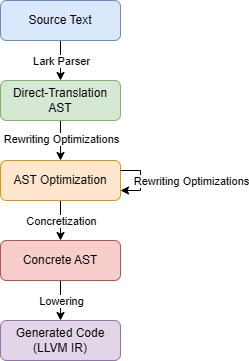
\includegraphics[width=.3\textwidth]{compiler_architecture.drawio.png}
%   \caption{Compiler pipeline, from plaintext source to LLVM IR}
%   \label{fig:compArch}
% \end{wrapfigure}

As the first step in processing the language, a CFG is used to convert plain text into a structured AST. For this draft, we have selected a grammar based on Python's familiar syntax \cite{pythonGrammar} and discrete mathematics based on a book by Gries and Schneider \cite{griesAndSchneider}. Aside from standardized language expression operators, control flow statements, and function definitions, the main features of this grammar are as follows:
\begin{itemize}
  \item Additional operators (and overloaded operators) dedicated to sets, sequences, and relations. With static typing, these will enable expressive statements closely resembling modelling specifications.
  \item Set construction-like comprehension statements for sets, sequences, and relations.
  \item Record types (structs) in place of classes, implemented as relations.
  \item Enums as static sets to collect names into a specific type. For example, when modelling a stop light intersection, the three stages of a light may be most clearly modelled as an enum with 3 states: red, yellow, and green.
\end{itemize}

The complete current grammar is available on \href{https://github.com/Ant13731/compilers/blob/main/implementation/grammar.lark}{GitHub}.

\subsubsection{AST and AST transformations}

The next step of our compiler is translating the CFG into a malleable AST. The Python library Lark \cite{lark} provides several choices of parsers, lexers, tree traversal methods, and top level interfaces to ease the process of parsing. From the grammar, Lark generates a generic AST \texttt{Transformer} that is traversable through methods corresponding to each grammar rule.

With the frontend of the compiler complete, we now move on to the optimization stage. This stage is perhaps the most complex to design and implement, since these decisions directly impact the balance of optimization capabilities and extensibility. For the subset of the language related to sets and set notation, we have implemented a simplified version of the rewrite strategy described at the end of Section 3.2. The current implementation collapses all sets connected by operators $\cup, \cap,$ and $\setminus$ into a single set connected by booleans. Then, generators are extracted from a list of candidates (ie. from the right side of the vertical bar in standard set notation, $p$ in the structure $\Set{x}{p}$). Unions, or ``or''-clauses within set notation, generally require two sequential set loops, while top-level ``and''-clauses for intersections and set differences share a single construction loop. Specifically, the prototype compiler is compliant with rewrite rules 1-4, 17, 21, and 23.

After rewriting terms to eliminate all superfluous operators, the compiler must decide on the best representation of data, given the context of relevant operations, object lifetimes, and expected memory usage. Finding generic optimizations across all possible use cases of data types may very well be undecidable, requiring complete knowledge of the code's runtime behaviours before the code has actually executed, but optimizing common operations may reach an acceptable level of improvement. We may further make use of modelling domain knowledge to heuristically optimize data representations (ex. bi-directional maps for the birthday book problem).

More concretely, LLVM defines several different types of sets that may be optimal depending on actions and expected size \cite{llvmSetDocs}. The built-in \texttt{SmallSet} saves large quantities of memory, for instance, but comes with linear access times. \texttt{Dense}- and \texttt{Sparse}-Sets on the other hand, provide access through hash tables and use more memory to prevent several \texttt{malloc} calls every insertion. Ordered elements within \texttt{Vector}s can enable extremely fast insertions and reasonably fast lookups. For our compiler, efficient lookups are preferred over efficient insertions, since we aim to trade intermediary set constructions for extra lookups for each element.

The remaining compilation step then lowers the optimized AST into LLVM IR. The Python library \texttt{llvmlite} \cite{llvmliteLib} provides APIs to generate IR statements directly from within Python, enabling straightforward code generation through tree traversals. However, since LLVM uses static single assignment form and C++ constructs for high efficiency, a post-optimization concrete AST may be necessary to replace chunks of the original AST with a closer-to-executable representation.

\section{Future Work}

Before we conclude this paper, it is important to illustrate two key points of research that should be resolved for a very high level language but are beyond the scope of this project.

In addition to set construction notation, we observed that a noticeable number of modelling examples make use of quantification logic within set generators. Currently, rewrite rules to optimize quantifier logic are not part of the Section 3 system. Instead, the language treats such expressions naively, looping over a given domain to find existential and universal quantification.

Second, generators for multiple variables within a comprehension must be optimized. A naive implementation may start with a double nested loop over both variable generators, however, any optimizations to reduce the number of superfluous loops will result in large leaps in runtime efficiency. Any opportunity to remove $O(n^2)$ and beyond code should be followed aggressively, but such a topic will need to be explored in detail, beyond the work of this current project.

\section{Conclusion}
The beginning stages of building a new programming language are arguably one of the most exciting and fundamental parts of the compiler development process. Exploring theoretical optimizations isolated from specific architectures and system limitations can lead to drastic improvements in overall performance with zero additional hardware costs. For our very high level language, we attempt to combine focused optimization techniques on a discrete mathematics language familiar to all computer scientists and software developers.


\pagebreak
\nocite{*} % keeps all references, even those not referred to
\printbibliography %Prints bibliography

\end{document}